%----------------------------------------------------------
\chapter{Архитектура программной реализации}\label{chap3_soft_architecture}
%----------------------------------------------------------
Проектирование новой программной архитектуры графового модуля библиотеки comsdk проводилось с учётом доступа разработчика к средствам стандартной библиотеки языка C++ стандарта C++-11 и библиотеки шаблонных классов Standart Template Library (STL).
\section{Узлы и рёбра графа}
Структура разработанных классов узла графа (\textsf{Node}) и ребра (\textsf{Edge}) представлена на рисунках \ref{fig:classNode}~и~\ref{fig:classEdge} соответственно.
\begin{figure}[!ht]
    \centering
    \begin{minipage}{0.455\textwidth}
        \centering
        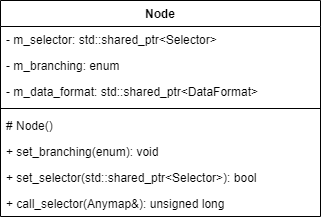
\includegraphics[width=0.9\textwidth]{figures/class.node.png}
        \caption{Класс узла графа}
        \label{fig:classNode}
    \end{minipage}\hfill
    \begin{minipage}{0.455\textwidth}
        \centering
        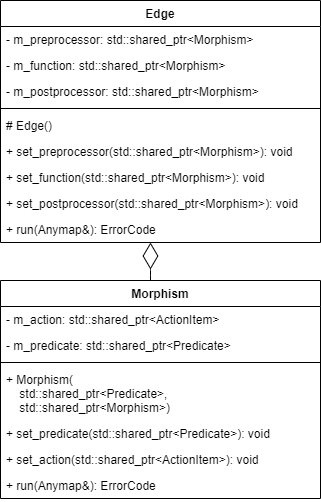
\includegraphics[width=0.9\textwidth]{figures/class.edge.png}
        \caption{Класс ребра графа}
        \label{fig:classEdge}
    \end{minipage}
\end{figure}

Как можно видеть, класс узла предоставляет интерфейс для назначения и вызова селектора и назначения стратегии распараллеливания выходящих из узла рёбер. Класс ребра предоставляет интефейс для назначения ему до трёх морфизмов и их выполнения, что в полной мере соответствует обозначенным в разделе~\ref{section:requirements} требованиям.

\section{Хранение узлов и рёбер графа}
Задача хранения данных узлов и рёбер была отведена непосредственно классу графа (\textsf{Graph}). Кроме того, данному классу была отведена задача хранить данные о топологии графовой модели в виде матрицы смежности. Данное решение позволяет легко проверять наличие ребра между двумя узлами и, кроме того, даёт возможность сразу узнать индекс ребра при его существовании. UML-диаграмма данного класса приведена на рисунке~\ref{fig:classGraph}.
\begin{figure}[!ht]
    \centering
    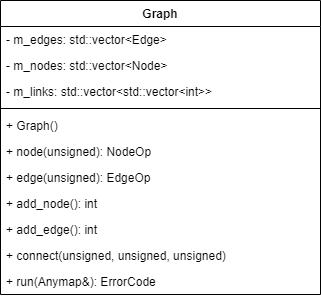
\includegraphics[height=6cm]{figures/class.graph.png}
    \caption{Класс графа}
    \label{fig:classGraph}
\end{figure}

Помимо этого для удобства доступа к структуре графа во время обхода были спроектированы две вспомогательные структуры данных, позволяющих отделить данные о топологии графа от отдельно взятых узлов и рёбер. UML-диаграммы этих структур представлены на рисунке~\ref{fig:additionalGraphStructure}.
\begin{figure}[!ht]
    \centering
    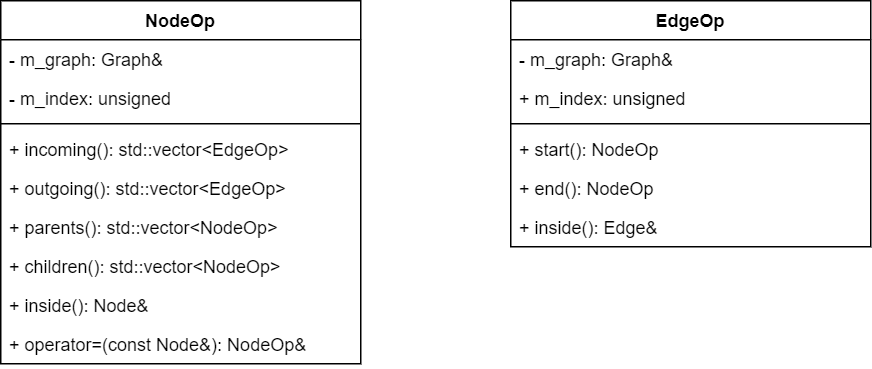
\includegraphics[height=5cm]{figures/structure_additional.png}
    \caption{Дополнительные структуры данных}
    \label{fig:additionalGraphStructure}
\end{figure}

Например, класс \textsf{NodeOp} предоставляет интерфейс для получения входящих и выходящих рёбер для конкретного узла, соседних узлов и при необходимости позволяет обратиться непосредственно к интерфейсу самого узла.

Итоговая UML-диаграмма классов, спроектированных в рамках графового модуля comsdk представлена на рисунке~\ref{fig:suggestedGraphStructure}.
\begin{figure}[!ht]
    \centering
    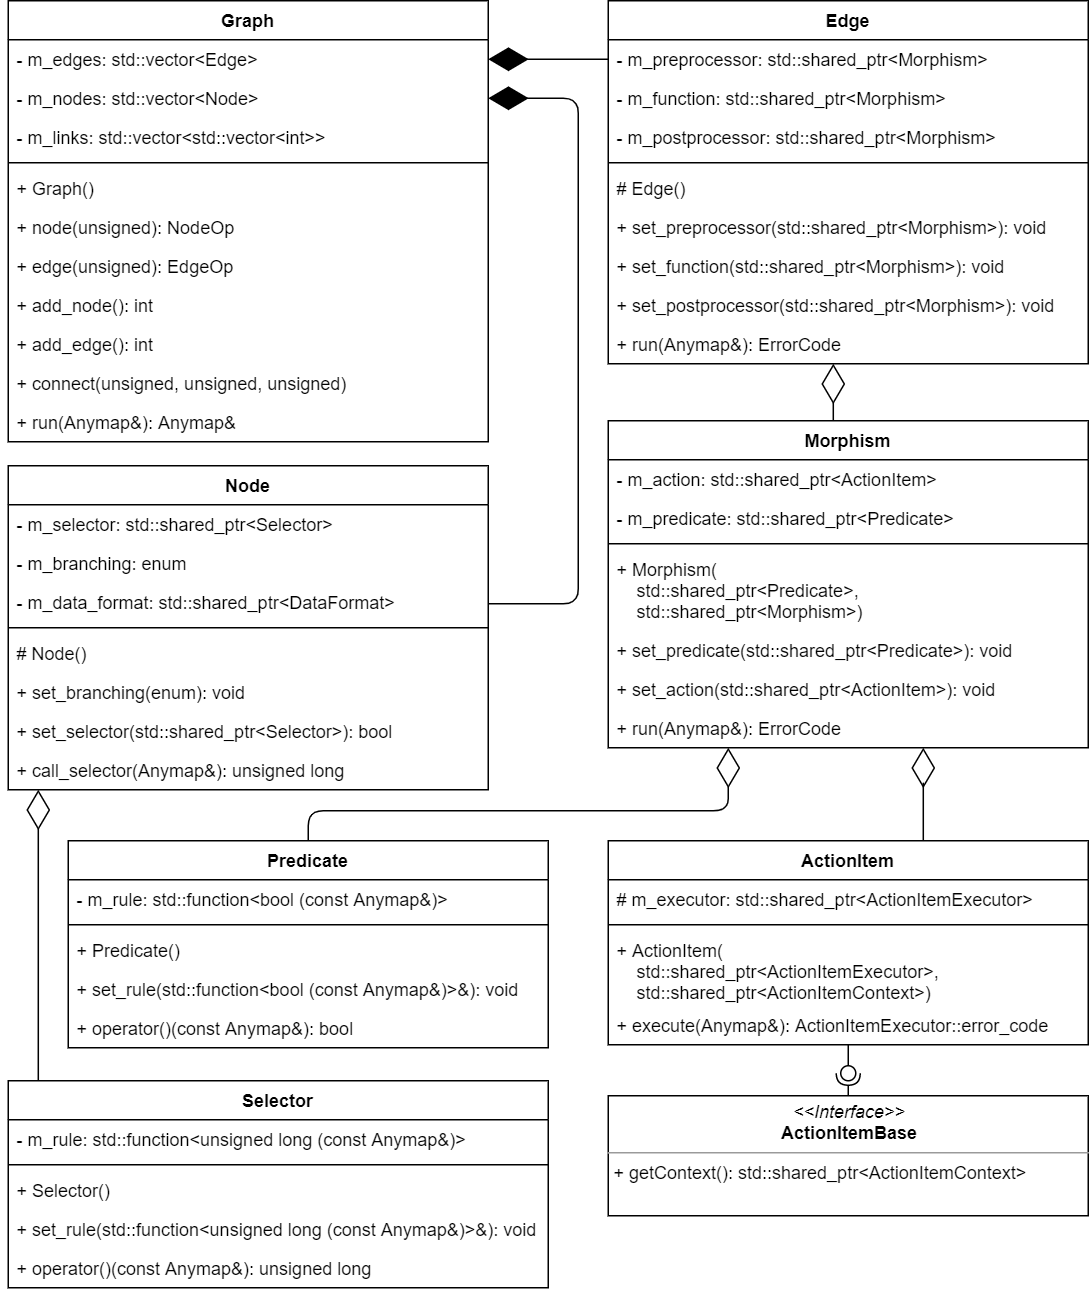
\includegraphics[width=\textwidth]{figures/suggested_structure.png}
    \caption{Предлагаемая структура классов}
    \label{fig:suggestedGraphStructure}
\end{figure}
%----------------------------------------------------------
%\section{...}

%----------------------------------------------------------

